\documentclass[a4paper,oneside]{article}
%Compilé avec MacTex
\usepackage[french]{babel}
\usepackage[utf8]{inputenc}
\usepackage{hyperref} % références dans pdf
\usepackage[tt]{titlepic}
\usepackage{graphicx} % pour images
\usepackage{rotating} % pour rotatebox
\usepackage{lmodern}
\usepackage{amsmath}
\usepackage{amssymb}
\usepackage{mathrsfs}
\usepackage{sistyle}
\usepackage{chngpage}
\usepackage{caption}
\usepackage{epstopdf}
\usepackage{gnuplottex}% pour faire du gnuplot directement dans le latex
\usepackage{listings}
\usepackage[nottoc, notlof, notlot]{tocbibind} % pour que bibliographie soit comprise comme un chapitre ou section
\usepackage{appendix} % pour les annexes
\pagestyle{headings} % pour en têtes
\usepackage{mathenv}
  %\usepackage{SIunitx}
%\usepackage{siunitx}%pour les unités SI
\DeclareTextSymbol{\degre}{OT1}{23} %pour le symbole degré
\makeatletter % pour /bigcenter qui permet de s'affranchir des marges pour les images
\newskip\@bigflushglue \@bigflushglue = -100pt plus 1fil

\def\bigcenter{\trivlist \bigcentering\item\relax}
\def\bigcentering{\let\\\@centercr\rightskip\@bigflushglue%
\leftskip\@bigflushglue
\parindent\z@\parfillskip\z@skip}
\def\endbigcenter{\endtrivlist}
\makeatother




\begin{document}
\lstset{language=Matlab,breaklines=true,keepspaces=true,                 % how far the line-numbers are from the code
  %numberstyle=\normal,numbers=left,                    % where to put the line-numbers; possible values are (none, left, right)
  %numbersep=5pt,   % the style that is used for the line-numbers
  frame=single, xleftmargin=2em}
\lstset{literate=
  {á}{{\'a}}1 {é}{{\'e}}1 {í}{{\'i}}1 {ó}{{\'o}}1 {ú}{{\'u}}1
  {Á}{{\'A}}1 {É}{{\'E}}1 {Í}{{\'I}}1 {Ó}{{\'O}}1 {Ú}{{\'U}}1
  {à}{{\`a}}1 {è}{{\`e}}1 {ì}{{\`i}}1 {ò}{{\`o}}1 {ù}{{\`u}}1
  {À}{{\`A}}1 {È}{{\'E}}1 {Ì}{{\`I}}1 {Ò}{{\`O}}1 {Ù}{{\`U}}1
  {ä}{{\"a}}1 {ë}{{\"e}}1 {ï}{{\"i}}1 {ö}{{\"o}}1 {ü}{{\"u}}1
  {Ä}{{\"A}}1 {Ë}{{\"E}}1 {Ï}{{\"I}}1 {Ö}{{\"O}}1 {Ü}{{\"U}}1
  {â}{{\^a}}1 {ê}{{\^e}}1 {î}{{\^i}}1 {ô}{{\^o}}1 {û}{{\^u}}1
  {Â}{{\^A}}1 {Ê}{{\^E}}1 {Î}{{\^I}}1 {Ô}{{\^O}}1 {Û}{{\^U}}1
  {Ã}{{\~A}}1 {ã}{{\~a}}1 {Õ}{{\~O}}1 {õ}{{\~o}}1
  {œ}{{\oe}}1 {Œ}{{\OE}}1 {æ}{{\ae}}1 {Æ}{{\AE}}1 {ß}{{\ss}}1
  {ű}{{\H{u}}}1 {Ű}{{\H{U}}}1 {ő}{{\H{o}}}1 {Ő}{{\H{O}}}1
  {ç}{{\c c}}1 {Ç}{{\c C}}1 {ø}{{\o}}1 {å}{{\r a}}1 {Å}{{\r A}}1
  {€}{{\euro}}1 {£}{{\pounds}}1 {«}{{\guillemotleft}}1
  {»}{{\guillemotright}}1 {ñ}{{\~n}}1 {Ñ}{{\~N}}1 {¿}{{?`}}1
}
 
%************************************************************************
%									TITRE
%************************************************************************


\begin{titlepage} % Suppresses headers and footers on the title page

	\centering % Centre everything on the title page

	\scshape % Use small caps for all text on the title page

	\vspace*{\baselineskip} % White space at the top of the page


	\rule{\textwidth}{1.6pt}\vspace*{-\baselineskip}\vspace*{2pt}
	 % Thick horizontal rule
	\rule{\textwidth}{0.4pt} % Thin horizontal rule

	\vspace{0.75\baselineskip} % Whitespace above the title

	{\LARGE Travaux Dirigés :\\
	\vspace{0.75\baselineskip}
	Test d'Adéquation\\
	} % Title

	\vspace{1\baselineskip} % Whitespace below the title
	\rule{\textwidth}{0.4pt}\vspace*{-\baselineskip}\vspace*{3.2pt}
	 % Thin horizontal rule
	\rule{\textwidth}{1.6pt} % Thick horizontal rule
	\vspace{2\baselineskip} % Whitespace after the title block

	%------------------------------------------------
	%	Subtitle
	%------------------------------------------------

	% Subtitle or further description
	Statistiques

	\vspace*{3\baselineskip} % Whitespace under the subtitle

	%------------------------------------------------
	%	Editor(s)
	%------------------------------------------------


	\vspace{0.5\baselineskip} % Whitespace before the editors

	{\scshape\Large Quentin Bergé \\} % Editor list

	\vspace{0.5\baselineskip} % Whitespace below the editor list

	\textit{ENSEEIHT} % Editor affiliation

	\vfill % Whitespace between editor names and publisher logo

	%------------------------------------------------
	%	Publisher
	%------------------------------------------------

	
\includegraphics[scale=0.8]{logoN7.png} % changer logo

	\vspace{0.3\baselineskip} % Whitespace under the publisher logo

Juin 2019 % Publication year
\end{titlepage}
\newpage

%Table des Matières
%\tableofcontents
%\newpage

\section{Introduction}

Le sujet de cette étude est d'observer pendant $n =$ 300 jours consécutifs de déterminer la loi de distribution de la variable aléatoire "absence de ceinture".
\section{Statistiques Descriptives}

\begin{enumerate}
  \item

  Pour construire l'histogramme des fréquences on a mis ceci dans Matlab.
  On a par la même occasion ajouté les valeurs extrêmes de la variable aléatoire.

\begin{lstlisting}

  % Figure 1
bar(Xemp,femp,'w')
hold on
plot(minX,femp(minXi),'x',maxX,femp(minXi),'o',Xemp(modefi),modef,'d') %plot des max et min et mode
plot(Xemp,ftheo,'r')

\end{lstlisting}


  \begin{figure}[h!]
  \bigcenter
  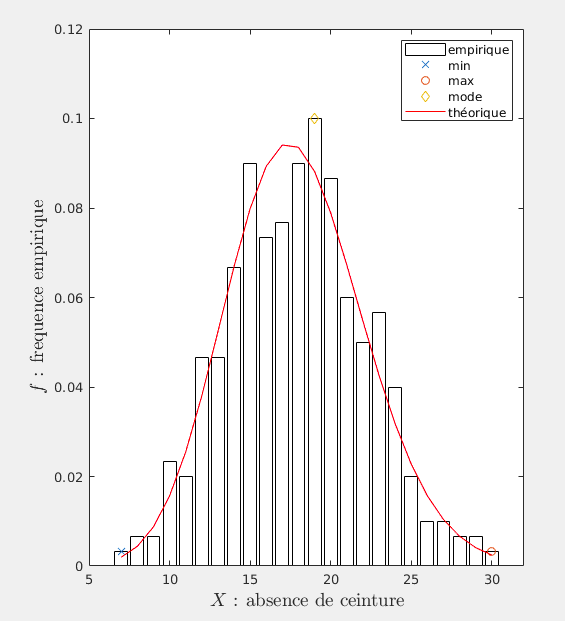
\includegraphics[scale=0.8]{fig_1_sub1.png}
  \caption{Histogramme des fréquences}
  \end{figure}


L'histogramme des fréquences paraît centré sur la moyenne et cela pourrait s'apparenter à une loi normale.

\clearpage

\item Afin d'obtenir les valeurs extrêmes de la v.a. on utilise les fonctions intrinsèques \verb?min? et \verb?max? qui nous donne la valeur maximale et minimale ainsi que l'indice de cette valeur.

\begin{lstlisting}
[maxX,maxXi]=max(Xemp); %on récupère le max des fréquence, ainsi que l'indice de ce max
[minX,minXi]=min(Xemp);
\end{lstlisting}

Nous utiliserons cet indice pour le tracer dans la figure avec la valeur maximale en abscisse, et la valeur de l'effectif empirique correspondante.
On obtient le minimum égal à 7 c'est-à-dire qu'au minimum il y a eu 7 absences de ceinture et qu'au maximum il y a eu 30 absences de ceinture de sécurité.\\

\item

Le mode correspond à la valeur la plus fréquente de l'effectif empirique.
Pour la trouver nous utilisons encore une fois la valeur maximale sur l'effectif empirique cette fois-ci.

\begin{lstlisting}
%Pour le mode c'est la valeur la plus fréquente => max de f
[modef,modefi]=max(femp);
\end{lstlisting}

On obtient le mode égal à 0.1, or $0.1\times 300 =30$, l'effectif associé est 19, que durant 30 jours il y a eu 19 absences de ceintures, c'est le nombre d'absences de ceintures que l'on trouve le plus fréquemment.
On le tracera de la même manière que précédemment dans la figure.\\

\item

Afin de construire et de tracer l'histogramme des fréquences cumulées ou fonction de répartition empirique (CDF) de la variable aléatoire, on effectue la somme cumulative des fréquences empiriques à l'aide d'une boucle.

\begin{lstlisting}
% calcul de la CDF empirique
CDF=zeros(1,n); %initialisation
CDF(1)=femp(1);
for i=2:n
    CDF(i)=CDF(i-1)+femp(i);
end
\end{lstlisting}


On le représente ensuite dans la figure suivante en implantant dans Matlab le code suivant :

\begin{lstlisting}
%Figure 2
bar(Xemp,CDF)%CDF empirique en barres
hold on
plot(Xemp(di1),CDF(di1),'o',Xemp(medi),CDF(medi),'d',Xemp(c95i),CDF(c95i),'x')
\end{lstlisting}

\begin{figure}[h!]
\bigcenter
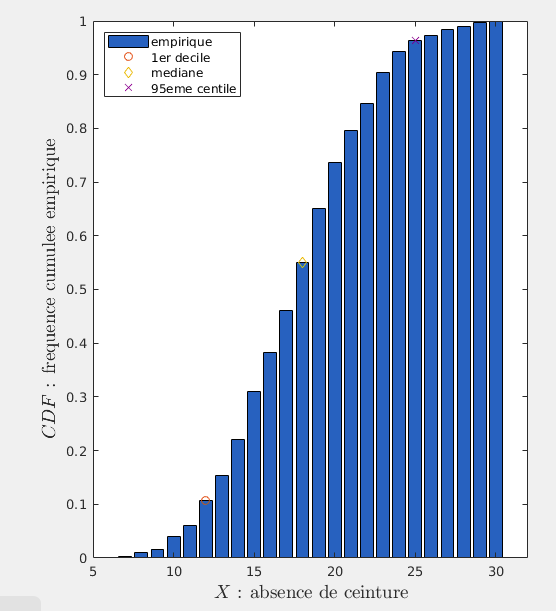
\includegraphics[scale=0.8]{fig1_sub2.png}
\caption{Histogramme des fréquences cumulées empiriques}
\end{figure}

\newpage
\item



Pour trouver les $1^{er}$ décile, la médiane et le $95^{\`eme}$ centile on va utiliser la fonction \verb?find? qui permet de renvoyer le premier indice de la valeur mise en argument.

\newpage
\begin{lstlisting}
%find renvoi direct l'indice
di1=find(CDF>0.1,1);%1er décile
medi=find(CDF>0.5,1);%mediane
c95i=find(CDF>0.95,1);%95 centile
\end{lstlisting}

On trouve le $1^{er}$ décile égal à 13, c'est-à-dire que 10 $\%$ des valeurs représentent 13 absences de ceintures.
La médiane est de 18, cela signifie que 18 absences de ceintures partagent la série en 2 parties du même effectif.
Le $95^{ème}$ centile est de 25, c'est-à-dire que 95 $\%$ des valeurs représentent 25 absences de ceintures.
\end{enumerate}


\section{Choix de la Théorie et Calculs des Paramètres}

\begin{enumerate}
  \item

La formule de la densité de probabilité d'une loi de poisson est :
  \[
\frac{\lambda^k}{k!} e^{- \lambda}
  \]

  \item

  Cette loi possède un paramètre qui est $\lambda$

  \item Calculons l'espérance mathématique de la loi de Poisson :

\[
 E(x) = \sum_{k=0}^{+\infty} k\frac{\lambda^k}{k!} e^{-\lambda}
\]
Or puisque pour $p(0) =  P(X = 0)= 0 \times \frac{\lambda^0}{0!} e^{- \lambda} =\ 0$, on peut commencer la somme à 1, Ainsi 

\[
 E(x) =  \sum_{k=1}^{+\infty} k\frac{\lambda^k}{k!} e^{- \lambda}\\
 \]
 \[
 E(x) =  \sum_{k=1}^{+\infty} \frac{k \lambda^k}{k!} e^{-\lambda}
 \]
 
 \[
 E(x) =  \sum_{k=1}^{+\infty} \frac{ \lambda^k}{(k-1)!} e^{- \lambda}\\
 \]
 \[
  E(x) =  \sum_{k=1}^{+\infty} \frac{ \lambda*\lambda^{k-1}}{(k-1)!} e^{- \lambda}\\
\]

Posons $y=k-1 \leftrightharpoons k=y+1$, Ainsi il vient

\[
	  E(x) =  \sum_{y=0}^{+\infty} \frac{ \lambda*\lambda^{k}}{y!} e^{- \lambda}\\
\]
\[	  
	    E(x) =  \lambda*\sum_{k=0}^{+\infty} \frac{ \lambda^{y}}{y!} e^{- \lambda}\\
\]
\[	    
	    E(x) = \lambda
\]

On a bien $E(x) = \lambda$

  \item

Afin de calculer la moyenne empirique de la variable aléatoire on utilise la formule suivante que l'on a implanté sur Matlab :

\begin{lstlisting}
  moy=sum(Xemp.*femp);
\end{lstlisting}

On trouve alors une moyenne de 17.9033, en moyenne il y a donc eu 17.9 absences de ceintures.\\

\item

Pour calculer ces paramètres on va utiliser la méthode des moments.

On calcule le premier moment de la loi probabilités :

\[
 m_1 = E(x) = f(\theta)
\]

On calcule alors l'équivalent empirique

\[
\overline{x}=\frac{1}{n} \sum_{x}^{+\infty} x_i = m_1
 \]

 On égalise les deux

\[
 f(\theta) =  E(x) = m_1
 \]

D'où $\lambda$ =  $m_1$ = 17.9033.


\end{enumerate}

\section{Calcul de la Statistique et Conclusion}

\begin{enumerate}

\item
On peut calculer alors le $\lambda$


\begin{lstlisting}
lambda=sum(Xemp.*femp);
\end{lstlisting}

Cela nous aidera à construire les fréquences théoriques à l'aide de la loi de poisson et l'effectif théorique :

\begin{lstlisting}
%Calcul de la fréquence theorique
ftheo=zeros(1,n);
for i=1:n
    ftheo(i)=lambda^Xemp(i)*exp(-lambda)/factorial(Xemp(i));
end

%Calcul de l'effectif théorique
tk=zeros(1,n);
tk=300.*ftheo;
\end{lstlisting}


\begin{center}
\begin{tabular}{|c|c|c|c|}

 \hline
 x	& effectif empirique & fréquence théorique & effectif thérorique\\
 \hline
 7 & 1	& 1,96E-03 & 0,589\\
 8 &	2	& 4,39E-03 & 1,318\\
 9 & 2	& 8,74E-03	&2,621\\
 10	&7	&1,56E-02	&4,692\\
 11	&6&	2,55E-02&	7,637\\
 12	&14	&3,80E-02&	11,394\\
 13	&14&	5,23E-02	&15,691\\
 14	&20	&6,69E-02	&20,066\\
 15	&27&	7,98E-02&23,950\\
 16	&22	&8,93E-02	&26,799\\
 17	&23&	9,41E-02	&28,223\\
 18	&27	&9,36E-02	&28,072\\
 19	&30&	8,82E-02	&26,452\\
 20	&26&	7,89E-02	&23,679\\
 21	&18&	6,73E-02	&20,187\\
 22	&15&	5,48E-02	&16,428\\
 23	&17&	4,26E-02	&12,788\\
 24	&12&	3,18E-02	&9,539\\
 25	&6	&2,28E-02	&6,831\\
 26	&3	&1,57E-02	&4,704\\
 27	&3	&1,04E-02	&3,119\\
 28	&2	&6,65E-03	&1,994\\
 29	&2 &4,10E-03	&1,231\\
 30	&1	&2,45E-03	&0,735\\
 \hline
 Total	&300	&0,996	&298,740\\

 \hline
\end{tabular}
\captionof{table}{Tableau rassemblant effectifs empiriques, les fréquences théoriques, ainsi que l'effectif théorique}
 \end{center}

\item

Pour calculer le nombre d'intervalles on va calculer la longueur de l'effectif théorique :

\begin{lstlisting}
% Il doit y avoir au moins 8 intervalles, ici il y en a 24 donc c'est bon
nb_intvl = length(tk);
\end{lstlisting}

On a ici 24 intervalles ce qui est bien supérieur à 8.\\


\item

Afin de trouver si l'effectif est assez important, il faudrait au moins que 80 $\%$ des valeurs soient supérieurs à 5.

Pour cela on va encore une fois utiliser la fonction \verb?find? comme ceci : 

\begin{lstlisting}
tk_5=find(tk>5);
int_80=length(tk_5)/length(tk);
\end{lstlisting}

Dans ce cas on obtient que les valeurs supérieures à 5 représentent 62.5 $\%$, ce qui est bien inférieur à 80 $\%$, donc l'effectif théorique n'est pas assez important dans les intervalles.

\newpage

\item
On veut enfin évaluer l'intégrale de la densité de probabilité sur son support. On réalise pour cela la somme des fréquences théoriques.

\begin{lstlisting}
int_ddp=sum(ftheo);

\end{lstlisting}

On trouve ici que l'intégrale de la densité de probabilité est égale à 0.9958 ce qui est différent de 1.

De plus, en souhaitant vérifier l'effectif théorique des observations :

\begin{lstlisting}
tk_tot = sum(tk);

\end{lstlisting}

On trouve alors \verb?tk_tot? égal à 298.7396 au lieu de 300.

On conclut donc qu'il doit nous manquer des valeurs.\\

\item

On regroupe alors pour parer le problème des valeurs extrêmes.


\begin{center}
\begin{tabular}{|c|c|c|c|}

 \hline
 x	& effectif empirique & fréquence théorique & effectif thérorique\\
 \hline
 inf. ou égal à 9 & 5	& 0.0162& 4.8617\\
 10 &	7	& 0.0156 & 4.6922\\
 11	& 	6	& 0.0255	&7.6369\\
 12	&	14	& 0.0380	&11.3939\\
 13	&	14  & 0.0523   &	15.6914\\
 14	&	20	& 0.0669 &	20.0664\\
 15	&	27  & 0.0798 &23.9503\\
 16	&	22	& 0.0893 &26.7994\\
 17	&	23  & 0.0941 &28.2235\\
 18	&	27	& 0.0936 &28.0719\\
 19	&	30  & 0.0882	 &26.4516\\
 20	&	26	& 0.0789 &23.6786\\
 21	&	18  & 0.0673	&20.1869\\
 22	&	15 &  0.0548	&16.4279\\
 23	&	17 & 0.0426	 &12.7876\\
 24	&	12 & 0.0318	&9.5392\\
 25	&	6  & 0.0228	&6.8313\\
 26 &	3 &	 0.0157 &4.7040\\
 27 et + &8	& 0.0267 &8.0054\\
\hline
 Total	&300	&1	&300.000\\

 \hline
\end{tabular}
\captionof{table}{Tableau rassemblant effectifs empiriques, les fréquences théoriques, ainsi que l'effectif théorique regroupés}
 \end{center}

\newpage

Pour calculer les fréquences théoriques empiriques on va utiliser les calculs suivants :

\begin{lstlisting}
%Calcul de la fréquence theorique apres regroupement "ftheo_reg"
ftheo_reg=zeros(length(X_reg),1);%initialisation

%Boucle pour remplir la 1ère valeur
for i=0:9 
    ftheo_reg(1)=lambda^i * exp(-lambda)/factorial(i)+ftheo_reg(1);
end

%Boucle pour remplir les valeurs du milieu
for i=2:19-1
   ftheo_reg(i)=lambda^X_reg(i) * exp(-lambda)/factorial(X_reg(i));
end    

%Pour remplir la 19ème valeur on prend la ddp=1 moins les autres valeurs
ftheo_reg(19) = 1-sum(ftheo_reg);
\end{lstlisting}


Ensuite on s'assure que la densité de probabilité après regroupement est égale à 1 :

\begin{lstlisting}
%somme des fréquences théoriques
	ddp_reg = sum(ftheo_reg);
\end{lstlisting}


On va alors calculer aussi l'effectif théorique après regroupement 

\begin{lstlisting}
tk_reg = 300.*ftheo_reg;
n_reg =sum(tk_reg);

\end{lstlisting}

On va s'assurer que l'effectif théorique regroupé est assez important dans les intervalles. Pour cela il faut au moins que 80 $\%$ des \verb?tk? soit supérieur à 5.

\begin{lstlisting}
tk_5_reg=find(tk_reg>=5);
inf_5_reg=length(tk_5_reg)/length(tk_reg);
\end{lstlisting}

\newpage
\item

On peut alors tracer les fréquences théoriques et empiriques selon le code suivant :

\begin{lstlisting}
	%Figure 3
bar(X_reg,femp_reg,'w')
plot(X_reg,ftheo_reg)
\end{lstlisting}

Ce qui donne ceci :

\begin{figure}[h!]
\bigcenter
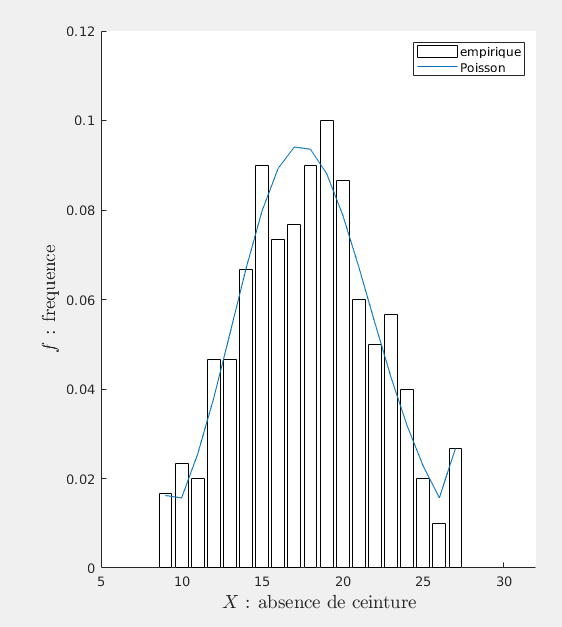
\includegraphics[scale=0.7]{fig2_sub1.png}
\caption{Histogramme des fréquences du regroupement}
\end{figure}

\pagebreak

On va pouvoir alors confronter les distributions empiriques et théoriques dans un diagramme de fréquences.

Pour ceci on va calculer la fonction de répartition empirique des observations regroupées :

\begin{lstlisting}
CDFemp_reg=zeros(length(X_reg),1);
CDFemp_reg(1)=1/n_theo_reg;
for i=2:19
    CDFemp_reg(i)=sum(femp_reg(1:i));
end
\end{lstlisting}


On va pouvoir aussi calculer la fonction de répartition de la loi de Poisson regroupée :

\begin{lstlisting}
CDFtheo_reg=zeros(length(X_reg),1);
CDFtheo_reg(1)=1/n_theo_reg;
for i=2:19
    CDFtheo_reg(i)=sum(ftheo_reg(1:i));
end
\end{lstlisting}


On pourra alors les tracer dans la figure 4 

\begin{lstlisting}
	%Figure 4
bar(X_reg,CDFemp_reg,'w')
plot(X_reg,CDFtheo_reg,'b')
\end{lstlisting}

%Ce qui donnera ceci :

\begin{figure}[h!]
\bigcenter
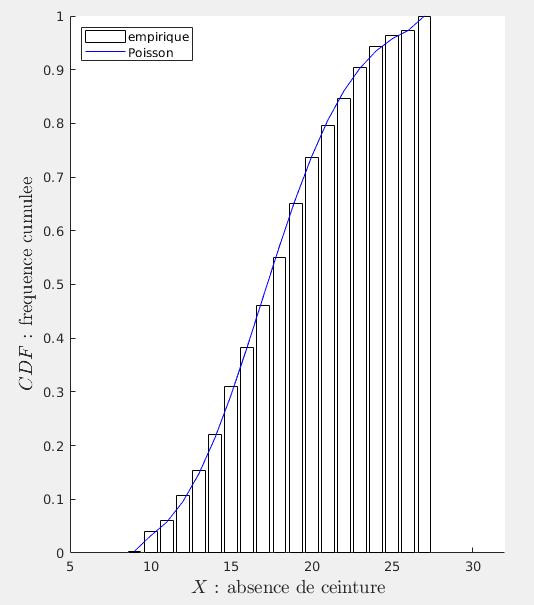
\includegraphics[scale=0.7]{fig2_sub2.png}
\caption{Histogramme des fréquences du regroupement}
\end{figure}
\newpage
\item

Pour comparer les écarts entre les distributions empiriques et théoriques on va calculer le $\chi^2$
selon la formule suivante :

\[
	\chi^2 = \sum_{k=1}^{k=n} \frac{(\theta_k - T_k)^2}{T_k}
\]
 que nous traduirons dans Matlab par le code suivant :
\begin{lstlisting}
	chi2 = sum((femp_reg.* n_theo_reg - tk_reg).^2 ./ tk_reg ) 
\end{lstlisting}

Cela nous donnera $\chi^2$ = 8.3295

\item

Si on fixe un risque $\alpha$ = 0.05, et que l'on a pour le calcul de degrés de liberté :
\[
	ddl = k - r - 1
\]

avec $r$ qui est le paramètre ici égal à 1 et $k$ égal à 19
cela nous donne donc 17 degrés de liberté.
Pour 17 degrés de liberté et un risque $\alpha$ on trouve un seuil de 27.857 dans la table du $\chi^2$.


\'Etant donné que le $\chi^2 < seuil$, on peut approuver l'hypothèse $H_0$ selon laquelle la loi de Poisson est une bonne loi théorique pour représenter le problème avec un risque de 5 $\%$ de se tromper.\\

\item

Avec le même nombre de degrés de liberté c'est-à-dire 17, on peut alors monter jusqu'à 95 $\%$ de risque.
\end{enumerate}


\end{document}
